ParMA defines the load transfer requirements for balancing a given entity
dimension based on the relative weight of the entities in neighboring parts.
Parts with an entity imbalance, $I^d_p$, greater than the specified imbalance, $tgtImb^d$,
are defined as heavily loaded parts.
A lightly loaded part is defined based on the partition improvement requirements.
If the application requires vertex$=$edge$>$element then migration to decrease
element imbalance should not increase the imbalance of vertices or edges.
Thus, during element improvement a part is a `lightly loaded' target to receive
elements if it has fewer vertices, edges and elements than the heavy part.

The amount of load, $l_{pq}^{d}$, migrated from a heavily loaded part $p$ to a
neighboring part $q$ during improvement of mesh entities of dimension $d$ is
defined as
\begin{equation}
  l_{pq}^{d}=\alpha*sf*\left( \sum_{i}{w(M^d_i \in p)} - \sum_{i}{w(M^d_i \in q)}\right) \text{,}
\label{eqn:migrW}
\end{equation}
where $w(M^d_i)$ is the application specified weight associated with a given
entity {\textit i}, $\alpha$ is a diffusion rate limiting constant $\in
(0,1]$~\cite{cybenko1989dynamic}, and, in 3D, $sf$ is
the ratio of mesh faces shared by parts $p$ and $q$ to the
total number of faces classified on partition boundaries of $p$.
The surface area bias $sf$ helps define load transfer requirements that can be
satisfied in a single iteration by selecting elements for migration that are
classified on the part boundary.
A large transfer across a small boundary will not only take several iterations
to satisfy, it will also lead to a large increase in the number of entities
classified on the part boundary as each iteration will `tunnel' into the part.
The entity selection process is detailed in Section~\ref{sec:entSelection}.


We tested the effect of $\alpha$ on run time and imbalance.
The test mesh of the automotive part shown in Fig.~\ref{fig:upright} has 2048
parts and an initial vertex imbalance of 46\%.
Table~\ref{tbl:alphaVsIterTime} and
Fig.~\ref{fig:alphaVsImb} respectively show the run time and vertex imbalance
as $\alpha$ is varied from 0.2 to 1.0.
Setting $\alpha$ to 0.6 yields the fewest iterations and the shortest run time.
Increasing $\alpha$ from this value causes too many elements to be migrated in
each iteration, which results in imbalance oscillations that increase the run
time.
Similarly, lower values of $\alpha$ increase the run time by migrating too few
elements in each iteration.
Given these observations, $\alpha$ is conservatively set to 0.5 for the
remaining tests in this work.

\begin{figure} [H] \centering
  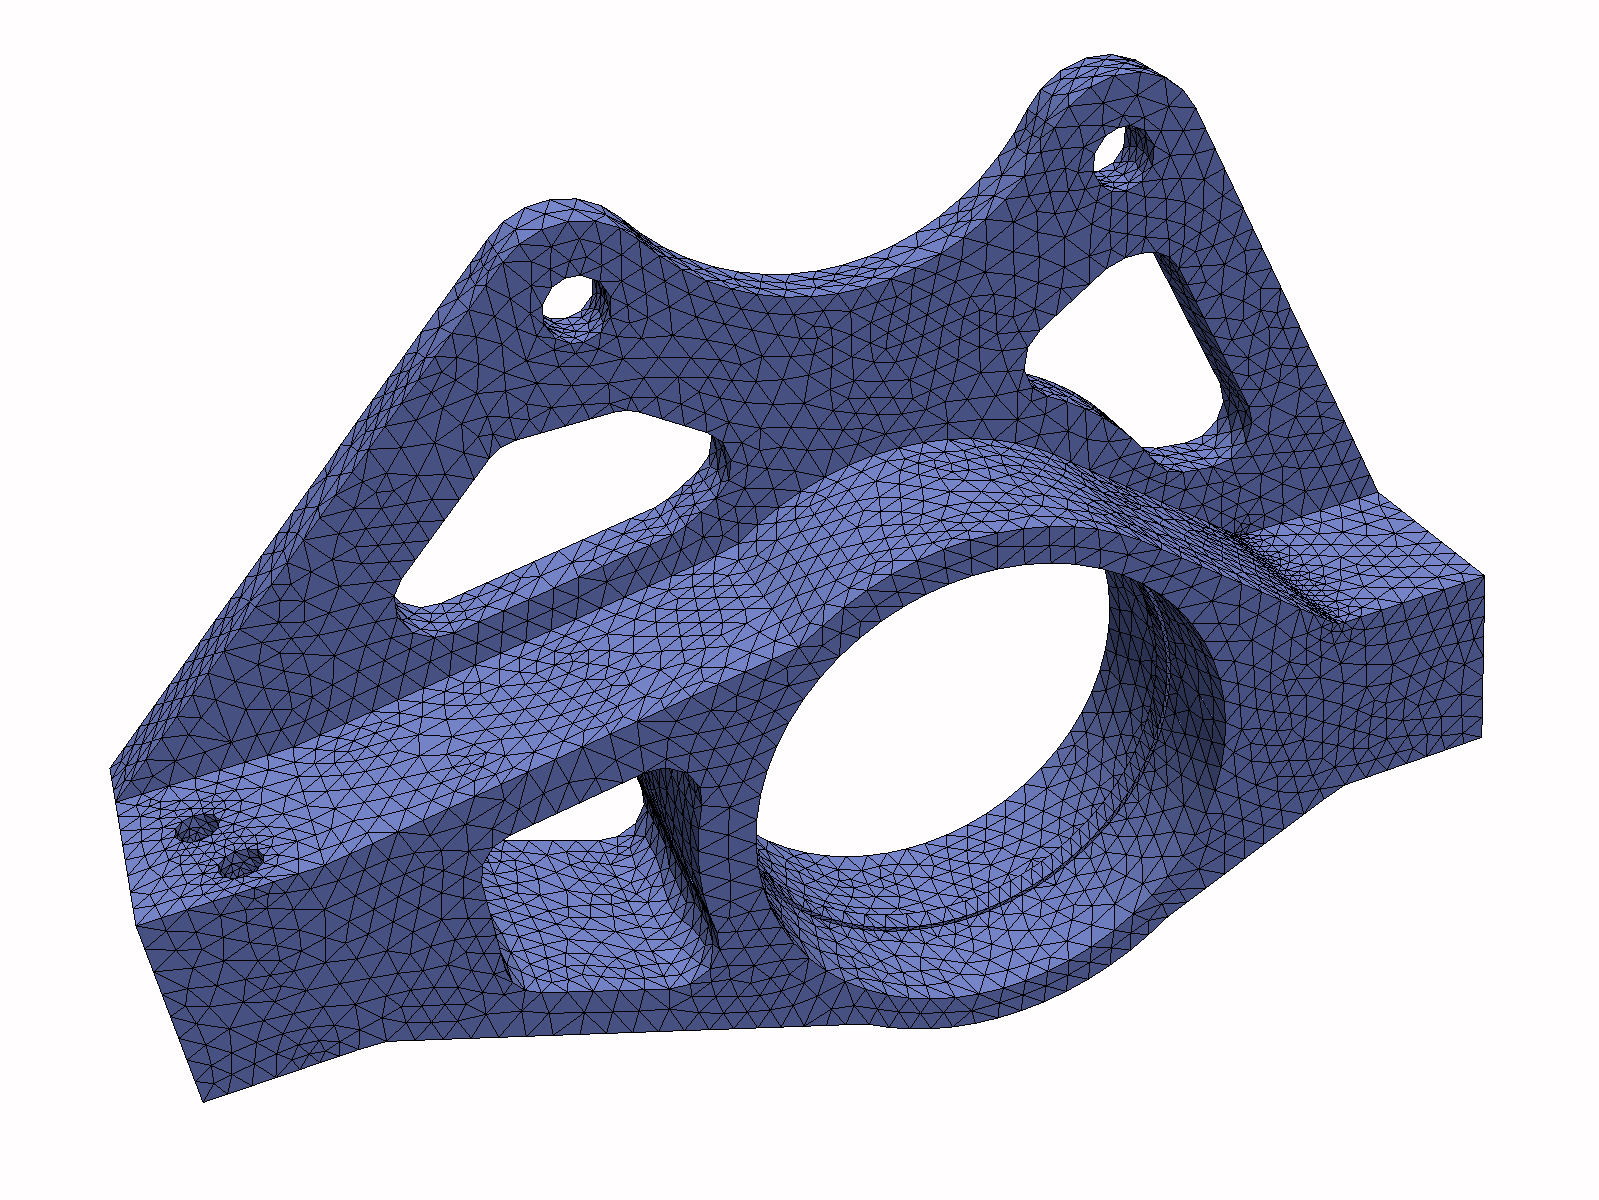
\includegraphics[width=.5\textwidth]{figs/upright-initial.png}
  \caption{
    Coarse mesh of the 2014 RPI Formula Hybrid suspension upright.
  }
  \label{fig:upright}
\end{figure}

\begin{figure} [H] \centering
  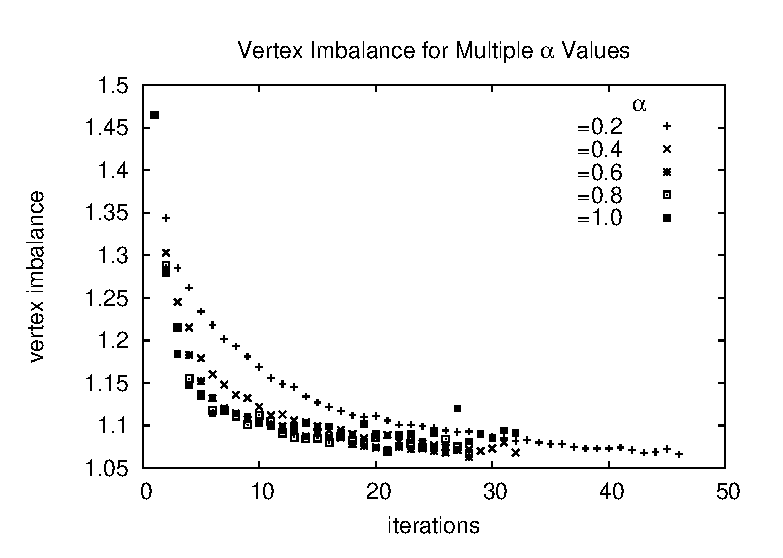
\includegraphics[width=.85\textwidth]{results/alpha/vtxImb.eps}
  \caption{
    Effects of $\alpha$ on the number of iterations, run time, and vertex imbalance.
    The initial mesh has 2048 parts and a 46\% vertex imbalance.
  }
  \label{fig:alphaVsImb}
\end{figure}

\begin{table} [H] \centering
  \small
  \caption{Diffusion iterations and run time for various $\alpha$ settings.}
  \label{tbl:alphaVsIterTime}
  \begin{tabular}{l | c F{4}{1} }
    $\alpha$ & iterations & {time (s)} \\
    \hline
    0.2 & 45 & 19.260470 \\
    0.4 & 31 & 13.990580 \\
    0.6 & 27 & 12.541773 \\
    0.8 & 27 & 13.502681 \\
    1.0 & 31 & 16.639643
  \end{tabular}
\end{table}


Compared to Zhou's LIIPBMod, ParMA's use of Equation~\ref{eqn:migrW} enables
finer grained migrations.
In LIIPBMod, a part is a target for migration if (1) the difference between the
vertex imbalance of the source part and the target part is greater than 2\% or
(2) the vertex imbalance is less than 4.5\%.
Note, LIIPBMod does not support weights associated with mesh vertices.
%numRgnRecv????  what is the transfer limit - ughhh the code does not match the
%paper
